\documentclass{article}

\usepackage[colorlinks=true, allcolors=blue]{hyperref}
\usepackage[english]{babel}
\usepackage[numbers]{natbib}
\usepackage{url}
\usepackage[utf8x]{inputenc}
\usepackage{amsmath}
\usepackage{graphicx}
\usepackage{parskip} 
\usepackage{fancyhdr}
\usepackage{vmargin}
\usepackage{tikz}
\usepackage{pgfplots} 
% \usepackage{minted}
\usepackage{placeins}
\usepackage{tikz}
\usepackage{titlesec}
\usepackage{caption}
\usepackage{subcaption}
 \usepackage[compatibility,siunitx,  americanvoltages, americancurrents, europeanresistors, europeaninductors, americanports,%
 straightlabels, fetbodydiode, straightvoltages]{circuitikz}
\usepackage{amssymb}
\usepackage{multirow}
\usepackage{siunitx}
\usepackage{pgfplots}
\usepackage{pgfgantt}
\usepackage{cleveref}

\usepackage{physics}
\usepackage{amsmath}
\usepackage{tikz}
\usepackage{mathdots}
\usepackage{yhmath}
\usepackage{cancel}
\usepackage{color}
\usepackage{siunitx}
\usepackage{array}
\usepackage{multirow}
\usepackage{amssymb}
\usepackage{gensymb}
\usepackage{tabularx}
\usepackage{extarrows}
\usepackage{booktabs}
\usetikzlibrary{fadings}
\usetikzlibrary{patterns}
\usetikzlibrary{shadows.blur}
\usetikzlibrary{shapes}




% \pgfplotsset{width=7cm,compat=1.3}
% \pgfplotsset{compat=newest}
% \pgfplotsset{plot coordinates/math parser=false} 
% \pgfplotsset{
%         % define the layers you need.
%         % (Don't forget to add `main' somewhere in that list!!)
%         layers/my layer set/.define layer set={
%             background,
%             main,
%             foreground
%         }{
%             % you could state styles here which should be moved to
%             % corresponding layers, but that is not necessary here.
%             % That is why we don't state anything here
%         },
%         % activate the newly created layer set
%         set layers=my layer set,
%     }

\input{Config/conf.tex}
% \newcommand{\Q}{Q1} 

\newenvironment{conditions}[1][where:]
  {#1 \begin{tabular}[t]{>{$}l<{$} @{${}={}$} l}}
  {\end{tabular}\\[\belowdisplayskip]}

\makeatletter
\renewcommand{\subsubsubsection}{\@startsection{paragraph}{4}{0ex}%
   {-3.25ex plus -1ex minus -0.2ex}%
   {1.5ex plus 0.2ex}%
   {\normalfont\normalsize\bfseries}}
\makeatother

\stepcounter{secnumdepth}
\stepcounter{tocdepth}


\makeatletter
% Save the original \section command
\let\oldsection\section
% Redefine the \section command to handle both optional arguments and the star variant
\renewcommand{\section}{\@ifstar{\mysectionstar}{\@ifnextchar[{\mysectionopt}{\mysection}}}
% Define the version of \section with a star (unnumbered)
\newcommand{\mysectionstar}[1]{%
  \def\currentsec{#1}% Update to use a more specific variable name
  \oldsection*{#1}%
}
% Define the version of \section with an optional argument
\newcommand{\mysectionopt}[2][]{%
  \def\currentsec{#2}% Update to use a more specific variable name
  \oldsection[#1]{#2}%
}
% Define the version of \section without an optional argument
\newcommand{\mysection}[1]{%
  \def\currentsec{#1}% Update to use a more specific variable name
  \oldsection{#1}%
}

% Assuming similar functionality is desired for \subsection,
% you would follow a similar pattern:
\let\oldsubsection\subsection
\renewcommand{\subsection}{\@ifstar{\mysubsectionstar}{\@ifnextchar[{\mysubsectionopt}{\mysubsection}}}
\newcommand{\mysubsectionstar}[1]{%
  \def\currentsubsec{#1}% Update to use a more specific variable name
  \oldsubsection*{#1}%
}
\newcommand{\mysubsectionopt}[2][]{%
  \def\currentsubsec{#2}% Update to use a more specific variable name
  \oldsubsection[#1]{#2}%
}
\newcommand{\mysubsection}[1]{%
  \def\currentsubsec{#1}% Update to use a more specific variable name
  \oldsubsection{#1}%
}
\makeatother

\newcommand{\inputsubsection}[1]{%
  \subsection{#1}%
  \documentclass{article}

\usepackage[colorlinks=true, allcolors=blue]{hyperref}
\usepackage[english]{babel}
\usepackage[numbers]{natbib}
\usepackage{url}
\usepackage[utf8x]{inputenc}
\usepackage{amsmath}
\usepackage{graphicx}
\usepackage{parskip} 
\usepackage{fancyhdr}
\usepackage{vmargin}
\usepackage{tikz}
\usepackage{pgfplots} 
% \usepackage{minted}
\usepackage{placeins}
\usepackage{tikz}
\usepackage{titlesec}
\usepackage{caption}
\usepackage{subcaption}
 \usepackage[compatibility,siunitx,  americanvoltages, americancurrents, europeanresistors, europeaninductors, americanports,%
 straightlabels, fetbodydiode, straightvoltages]{circuitikz}
\usepackage{amssymb}
\usepackage{multirow}
\usepackage{siunitx}
\usepackage{pgfplots}
\usepackage{pgfgantt}
\usepackage{cleveref}

\usepackage{physics}
\usepackage{amsmath}
\usepackage{tikz}
\usepackage{mathdots}
\usepackage{yhmath}
\usepackage{cancel}
\usepackage{color}
\usepackage{siunitx}
\usepackage{array}
\usepackage{multirow}
\usepackage{amssymb}
\usepackage{gensymb}
\usepackage{tabularx}
\usepackage{extarrows}
\usepackage{booktabs}
\usetikzlibrary{fadings}
\usetikzlibrary{patterns}
\usetikzlibrary{shadows.blur}
\usetikzlibrary{shapes}




% \pgfplotsset{width=7cm,compat=1.3}
% \pgfplotsset{compat=newest}
% \pgfplotsset{plot coordinates/math parser=false} 
% \pgfplotsset{
%         % define the layers you need.
%         % (Don't forget to add `main' somewhere in that list!!)
%         layers/my layer set/.define layer set={
%             background,
%             main,
%             foreground
%         }{
%             % you could state styles here which should be moved to
%             % corresponding layers, but that is not necessary here.
%             % That is why we don't state anything here
%         },
%         % activate the newly created layer set
%         set layers=my layer set,
%     }

\input{Config/conf.tex}
% \newcommand{\Q}{Q1} 

\newenvironment{conditions}[1][where:]
  {#1 \begin{tabular}[t]{>{$}l<{$} @{${}={}$} l}}
  {\end{tabular}\\[\belowdisplayskip]}

\makeatletter
\renewcommand{\subsubsubsection}{\@startsection{paragraph}{4}{0ex}%
   {-3.25ex plus -1ex minus -0.2ex}%
   {1.5ex plus 0.2ex}%
   {\normalfont\normalsize\bfseries}}
\makeatother

\stepcounter{secnumdepth}
\stepcounter{tocdepth}


\makeatletter
% Save the original \section command
\let\oldsection\section
% Redefine the \section command to handle both optional arguments and the star variant
\renewcommand{\section}{\@ifstar{\mysectionstar}{\@ifnextchar[{\mysectionopt}{\mysection}}}
% Define the version of \section with a star (unnumbered)
\newcommand{\mysectionstar}[1]{%
  \def\currentsec{#1}% Update to use a more specific variable name
  \oldsection*{#1}%
}
% Define the version of \section with an optional argument
\newcommand{\mysectionopt}[2][]{%
  \def\currentsec{#2}% Update to use a more specific variable name
  \oldsection[#1]{#2}%
}
% Define the version of \section without an optional argument
\newcommand{\mysection}[1]{%
  \def\currentsec{#1}% Update to use a more specific variable name
  \oldsection{#1}%
}

% Assuming similar functionality is desired for \subsection,
% you would follow a similar pattern:
\let\oldsubsection\subsection
\renewcommand{\subsection}{\@ifstar{\mysubsectionstar}{\@ifnextchar[{\mysubsectionopt}{\mysubsection}}}
\newcommand{\mysubsectionstar}[1]{%
  \def\currentsubsec{#1}% Update to use a more specific variable name
  \oldsubsection*{#1}%
}
\newcommand{\mysubsectionopt}[2][]{%
  \def\currentsubsec{#2}% Update to use a more specific variable name
  \oldsubsection[#1]{#2}%
}
\newcommand{\mysubsection}[1]{%
  \def\currentsubsec{#1}% Update to use a more specific variable name
  \oldsubsection{#1}%
}
\makeatother

\newcommand{\inputsubsection}[1]{%
  \subsection{#1}%
  \input{Src/\currentsec/\currentsubsec/main.tex}%
}

\newcommand{\inputsubsubsection}[1]{%
  \subsubsection{#1}%
  \input{Src/\currentsec/\currentsubsec/#1.tex}%
}

\newcommand{\Diagram}[2]{%
  \begin{figure}[h]
    \centering
    \includegraphics[width=0.8\textwidth]{Src/\currentsec/\currentsubsec/#1}
    \caption{#2}
    \label{fig:#1}
  \end{figure}
  \FloatBarrier
}
% Language setting
% Replace `english' with e.g. `spanish' to change the document language
\usepackage[english]{babel}

% Set page size and margins
% Replace `letterpaper' with `a4paper' for UK/EU standard size
% \usepackage[letterpaper,top=2cm,bottom=2cm,left=3cm,right=3cm,marginparwidth=1.75cm]{geometry}

% Useful packages
\usepackage{amsmath}
\usepackage{graphicx}
\usepackage[colorlinks=true, allcolors=blue]{hyperref}
\usepackage[cc]{titlepic}


% \title{Project Planing Report - Realisation of an Self Calibrating, Robust Adaptive Unscented Kalman Filter (RAUKF) based 3D Wind Variometer \\
% \includegraphics[width=\textwidth]{a.png}}

% \title{ Project Planing Report - Realisation of an Self Calibrating, Robust Adaptive Unscented Kalman Filter (RAUKF) based 3D Wind Variometer \\ \vspace{0.5cm}
% \includegraphics[width=0.5\textwidth]{a.jpg} 
% }






% \author{George Downing}

\begin{document}

\begin{titlepage}
    \centering
    %\vspace*{0.5 cm}
    
\includegraphics[scale = 0.4]{Config/uon.png}\\[1.0 cm]	% University Logo

    
    \textsc{\Large Department of Electrical and Electronic Engineering
    Faculty of Engineering}\\[0.5 cm]	% University Name
    \textsc{\large EEE Final Year Individual Project}\\[0.5 cm]				% Course Code
    \textsc{\large (EEEE4008 UNUK FYR) (24-25)}\\[0.5 cm]				% Course Name

    \rule{\linewidth}{0.2 mm} \\[0.4 cm]
    { \huge \bfseries \thetitle}\\
    \rule{\linewidth}{0.2 mm} \\[0.5 cm]

    \includegraphics[scale = 0.3]{Config/a.jpg}\\[1.0 cm]

    \large \emph{Author:} \theauthor \\[0.5 cm]


    {\large \thedate}\\[0 cm]

    \vfill

\end{titlepage}

% \section{Overleaf Hints (to be deleted later)}

% \subsection{jumping between doc and latex}
% use ctr+click to jump in pages. \\

% use ctr+S to compile document.


% \subsection{Drawings}
% make drawings with: https://www.mathcha.io/editor/ \\


% \subsection{Graphs}
% all graphs should be done in matlab. Use matlab2tikz to create a latex file:

% https://uk.mathworks.com/matlabcentral/fileexchange/22022-matlab2tikz-matlab2tikz

% use the command to add your graph: 
% \begin{verbatim}
%         \input{path/to/your/file.tex}
% \end{verbatim}  

% This should be wrapped in a figure see \cref{sub:figures}

% \subsection{Tables}
% to make tables use: 
% https://www.tablesgenerator.com/

% use the [ht!] flag to specify table position.\\

% use following to ensure it stays in bounds
% \begin{verbatim}
%     \centering
%     \resizebox{\columnwidth}{!}
% \end{verbatim}

% if wraparound boxes are needed use:
% \begin{verbatim}
%     \tabular{p{100}} where p 100 is in pt.
% \end{verbatim}\\

% see \cref{tab:inital_spec_vs_Considerations} for example\\

% \subsection{Peer Review process}
% leave in green, for someone else to read. don't click accept on your own work \\

% if you see green that is not your own work. review it, then accept it. make sure to use a spell checker (you can get Grammarly for overleaf)\\

% \subsection{figures} \label{sub:figures}
% please use the following template for figures:

% \begin{figure}[ht!]
%     \centering
%     % \includegraphics{}
%     \caption{Caption}
%     \label{fig:enter-label}
% \end{figure}


% \subsection{referencing}
% \subsubsection{Cross referencing}

% use \verb|\Cref and \cref| ... eg \Cref{tab:inital_spec_vs_Considerations} and \cref{tab:inital_spec_vs_Considerations}

% label where appropriate:

% eg: \verb|\label{fig:figure_descritpion}| or \verb|\label{tab:table_description}| or \verb|\label{sec:section_name}|

% \subsubsection{citations}

% get extension BibItNow:

% https://addons.mozilla.org/en-US/firefox/addon/bibitnow/

% copy reference in bibtex format.

% paste in file biblist.bib found in the main file tree near bottom.

% eg:

% \begin{verbatim}
%     @misc{CanoeSlalom,
% 	title = {{Canoe Slalom}},
% 	journal = {ICF - Planet Canoe},
% 	year = {2023},
% 	month = oct,
% 	note = {[Online; accessed 31. Oct. 2023]},
% 	url = {https://www.canoeicf.com/disciplines/canoe-slalom}
% }
% \end{verbatim}


% Then use \verb|\cite{CanoeSlalom}| to reference: \cite{CanoeSlalom}

% if done correctly it should automatically appear hyper linked to the bottom of the document.



% \pagebreak
% \vspace*{\fill}
% \begin{abstract}
%    This report will discuss the feasibility of creating a full slalom canoe and kayak timing and scoring systems to automate the adjudication of the water sport. The report investigates the background and context behind the sport, including looking at existing solutions and analysing where similar automation has been achieved in other sporting disciplines. The stakeholder's requirements have been analysed qualitatively and quantitatively to generate a set of specifications for initial idea generation. An IoT radio localisation system has been conceptualised to map, track and report the athlete's position in time and space. Satellite nodes on each pole contain sensors to detect hits and act as radio beacons for localisation and data communication. An offline computer processes this data to generate scoring and timing data, displayed in real-time to a spectator through an app. Subsystems for rover and satellite prototypes, as well as a prototype scoring system and application, were implemented and tested. The prototypes were analysed against the specifications and original stakeholder requirements. Reflections were made on all aspects of the project and the project as a whole, including project management. Areas for future work and further development proposed. Broader context and commercialisation strategies were discussed to extrapolate the work's long-term implications. 
% \end{abstract}
% \vspace*{\fill}
% \pagebreak
\pagebreak



\section{Project Overview}  %5
Student provides an overview of the main project aim that clearly and concisely sets out what the project must achieve and the importance of the work. A diagram is included that shows consideration of the main system components (hardware and/or software) or processes and how these are interconnected.

Project overview makes use of suitable references to support the engineering context of the project (e.g. use of academic papers for key concepts that will be applied).

Project overview makes use of suitable references to support the commercial context of the project (e.g. using market data to show consumer demand).

The project diagram makes good use of stylistic features (colour, font styles, groupings, shapes, etc) to intuitively separate sub-systems and components within the overall project. Use of styles are consistent.

Project diagram demonstrates complete understanding of critical component level design requirements (for example a MCU block might include peripheral/memory/clock needs, software routines may include API, algorithm, limitations, data type, execution time requirements).

The project diagram clearly shows, and where necessary explains, dependency between parts.
\section{Originality}   % 25
Student provides a suitable explanation of the originality of the project, highlighting where it fits within commercial/scientific context along with differentiating from existing intellectual property.
Student provides a suitable explanation of the originality of the project and attempts to demonstrate the need for this through assessment of the current commercial/scientific context.

The need for the project is clearly identified through assessment of both the wider background and a comparative look at existing IP/current practice. There is clear differentiation from existing IP/current practice.

Student acknowledges the limitations their project will have when compared to other work (e.g. less comprehensive testing facilities, only prototype manufacturing equipment). These are both discussed and justified with relation to originality. Student can quantify and extrapolate the impact of the limitations to their project specification.

Student explains project originality not only in the final deliverable, but also in the development approach.

Multifaceted novelty combining two or more of: new technique/approach/algorithm, interdisciplinary approach, translation from one technology area to others, low-cost solution with comparable performance to current practice.
\section{Specification} % 7.5
Student provides a list of relevant requirements for the final project deliverable that can be used to measure the success of the project. Specification points are suitably prioritised with additional requirements over the main aim given as “stretch goals” and grouped in a suitable way for the project (for example splitting hardware and software requirements).

Specification points are all quantitatively justified with respect to the project aim(s) and wider literature (e.g. H&S, legal requirements, engineering standards, best practice, etc). With inclusion of suitable references.

There is clear assessment of the expected challenge posed by each specification point.

Each requirement includes a succinctly clear explanation of how it will be tested including the criteria for success.

Specifications are shown to be both attainable (with the facilities available to the student) and realistic (in terms of the time frame of the project).  

Clear ambition to achieve specification beyond commercial-off-the-shelf or state-of-the-art research-grade system. There is evidence that such ambition is realisable. 
\section{Methodology}   % 7.5
Student provides a suitable development process for the project, highlighting some key tools and components that will be used within each step, and outlining the obvious limitations related to these. Selected tools are suitably justified with respect to the project aim/specification/ /time/etc.

Discussion of the implications of inter-dependencies between different steps.

Each step of the methodology is assessed in terms of the challenge posed to the student based on their individual experience and skill set. Additional tasks related to these are explained (e.g. use of a piece of software may require additional tasks to become familiar).

Limitations are explained and assessed with relation to the project development (e.g. using a licenced software may incur cost but be beneficial if the student already has experience).

Student effectively combines/synthesizes/translates existing methodologies leading to a bespoke solution which meets the specifications and accounts for all limitations.
\section{Risk Management and mitigation} %15
Student provides a list of some obvious expected risks that could impact completion of the project with inclusion of risks that are specific to the project methodology. Risks are accompanied by suitable mitigation actions.

The potential impact of risks on the project are realistically quantified in terms of time/cost/change in spec. Risks are sorted by impact.

Mitigation actions are realistic given the resources available to the project.

The likelihood of risks occurring are quantified with a method applied to sort the importance of each risk.

There is clear indication of when each risk is likely to occur in the project and this is considered as part of the mitigation actions.

All critical risks to the project are fully mitigated and quantified (rated) pre and post mitigation.
\section{Time Plan} %15
Student provides a Gantt chart that outlines the expected progress of the project, broken down into major tasks with completion points of deliverables and milestones indicated on chart. Gantt chart includes stages at which progress reviews will be carried out with an explanation is given for where the project is expected to be at each review.

Dependency between tasks is clearly indicated and explained.

Clear link of Gantt chart tasks to project specification and methodology.

Gantt chart and explanation demonstrates consideration of risks and mitigations with use of parallelisation.

Gantt chart has a visible cycle of develop, test, document.

Realistic time planning and work loading (based on # hrs per week).

Gantt chart demonstrates points of uncertainty (e.g. via error bars) and the impact on following tasks is explained.
% interview 15



\pagebreak
\end{document}%
}

\newcommand{\inputsubsubsection}[1]{%
  \subsubsection{#1}%
  \input{Src/\currentsec/\currentsubsec/#1.tex}%
}

\newcommand{\Diagram}[2]{%
  \begin{figure}[h]
    \centering
    \includegraphics[width=0.8\textwidth]{Src/\currentsec/\currentsubsec/#1}
    \caption{#2}
    \label{fig:#1}
  \end{figure}
  \FloatBarrier
}
% Language setting
% Replace `english' with e.g. `spanish' to change the document language
\usepackage[english]{babel}

% Set page size and margins
% Replace `letterpaper' with `a4paper' for UK/EU standard size
% \usepackage[letterpaper,top=2cm,bottom=2cm,left=3cm,right=3cm,marginparwidth=1.75cm]{geometry}

% Useful packages
\usepackage{amsmath}
\usepackage{graphicx}
\usepackage[colorlinks=true, allcolors=blue]{hyperref}
\usepackage[cc]{titlepic}


% \title{Project Planing Report - Realisation of an Self Calibrating, Robust Adaptive Unscented Kalman Filter (RAUKF) based 3D Wind Variometer \\
% \includegraphics[width=\textwidth]{a.png}}

% \title{ Project Planing Report - Realisation of an Self Calibrating, Robust Adaptive Unscented Kalman Filter (RAUKF) based 3D Wind Variometer \\ \vspace{0.5cm}
% \includegraphics[width=0.5\textwidth]{a.jpg} 
% }






% \author{George Downing}

\begin{document}

\begin{titlepage}
    \centering
    %\vspace*{0.5 cm}
    
\includegraphics[scale = 0.4]{Config/uon.png}\\[1.0 cm]	% University Logo

    
    \textsc{\Large Department of Electrical and Electronic Engineering
    Faculty of Engineering}\\[0.5 cm]	% University Name
    \textsc{\large EEE Final Year Individual Project}\\[0.5 cm]				% Course Code
    \textsc{\large (EEEE4008 UNUK FYR) (24-25)}\\[0.5 cm]				% Course Name

    \rule{\linewidth}{0.2 mm} \\[0.4 cm]
    { \huge \bfseries \thetitle}\\
    \rule{\linewidth}{0.2 mm} \\[0.5 cm]

    \includegraphics[scale = 0.3]{Config/a.jpg}\\[1.0 cm]

    \large \emph{Author:} \theauthor \\[0.5 cm]


    {\large \thedate}\\[0 cm]

    \vfill

\end{titlepage}

% \section{Overleaf Hints (to be deleted later)}

% \subsection{jumping between doc and latex}
% use ctr+click to jump in pages. \\

% use ctr+S to compile document.


% \subsection{Drawings}
% make drawings with: https://www.mathcha.io/editor/ \\


% \subsection{Graphs}
% all graphs should be done in matlab. Use matlab2tikz to create a latex file:

% https://uk.mathworks.com/matlabcentral/fileexchange/22022-matlab2tikz-matlab2tikz

% use the command to add your graph: 
% \begin{verbatim}
%         \input{path/to/your/file.tex}
% \end{verbatim}  

% This should be wrapped in a figure see \cref{sub:figures}

% \subsection{Tables}
% to make tables use: 
% https://www.tablesgenerator.com/

% use the [ht!] flag to specify table position.\\

% use following to ensure it stays in bounds
% \begin{verbatim}
%     \centering
%     \resizebox{\columnwidth}{!}
% \end{verbatim}

% if wraparound boxes are needed use:
% \begin{verbatim}
%     \tabular{p{100}} where p 100 is in pt.
% \end{verbatim}\\

% see \cref{tab:inital_spec_vs_Considerations} for example\\

% \subsection{Peer Review process}
% leave in green, for someone else to read. don't click accept on your own work \\

% if you see green that is not your own work. review it, then accept it. make sure to use a spell checker (you can get Grammarly for overleaf)\\

% \subsection{figures} \label{sub:figures}
% please use the following template for figures:

% \begin{figure}[ht!]
%     \centering
%     % \includegraphics{}
%     \caption{Caption}
%     \label{fig:enter-label}
% \end{figure}


% \subsection{referencing}
% \subsubsection{Cross referencing}

% use \verb|\Cref and \cref| ... eg \Cref{tab:inital_spec_vs_Considerations} and \cref{tab:inital_spec_vs_Considerations}

% label where appropriate:

% eg: \verb|\label{fig:figure_descritpion}| or \verb|\label{tab:table_description}| or \verb|\label{sec:section_name}|

% \subsubsection{citations}

% get extension BibItNow:

% https://addons.mozilla.org/en-US/firefox/addon/bibitnow/

% copy reference in bibtex format.

% paste in file biblist.bib found in the main file tree near bottom.

% eg:

% \begin{verbatim}
%     @misc{CanoeSlalom,
% 	title = {{Canoe Slalom}},
% 	journal = {ICF - Planet Canoe},
% 	year = {2023},
% 	month = oct,
% 	note = {[Online; accessed 31. Oct. 2023]},
% 	url = {https://www.canoeicf.com/disciplines/canoe-slalom}
% }
% \end{verbatim}


% Then use \verb|\cite{CanoeSlalom}| to reference: \cite{CanoeSlalom}

% if done correctly it should automatically appear hyper linked to the bottom of the document.



% \pagebreak
% \vspace*{\fill}
% \begin{abstract}
%    This report will discuss the feasibility of creating a full slalom canoe and kayak timing and scoring systems to automate the adjudication of the water sport. The report investigates the background and context behind the sport, including looking at existing solutions and analysing where similar automation has been achieved in other sporting disciplines. The stakeholder's requirements have been analysed qualitatively and quantitatively to generate a set of specifications for initial idea generation. An IoT radio localisation system has been conceptualised to map, track and report the athlete's position in time and space. Satellite nodes on each pole contain sensors to detect hits and act as radio beacons for localisation and data communication. An offline computer processes this data to generate scoring and timing data, displayed in real-time to a spectator through an app. Subsystems for rover and satellite prototypes, as well as a prototype scoring system and application, were implemented and tested. The prototypes were analysed against the specifications and original stakeholder requirements. Reflections were made on all aspects of the project and the project as a whole, including project management. Areas for future work and further development proposed. Broader context and commercialisation strategies were discussed to extrapolate the work's long-term implications. 
% \end{abstract}
% \vspace*{\fill}
% \pagebreak
\pagebreak



\section{Project Overview}  %5
Student provides an overview of the main project aim that clearly and concisely sets out what the project must achieve and the importance of the work. A diagram is included that shows consideration of the main system components (hardware and/or software) or processes and how these are interconnected.

Project overview makes use of suitable references to support the engineering context of the project (e.g. use of academic papers for key concepts that will be applied).

Project overview makes use of suitable references to support the commercial context of the project (e.g. using market data to show consumer demand).

The project diagram makes good use of stylistic features (colour, font styles, groupings, shapes, etc) to intuitively separate sub-systems and components within the overall project. Use of styles are consistent.

Project diagram demonstrates complete understanding of critical component level design requirements (for example a MCU block might include peripheral/memory/clock needs, software routines may include API, algorithm, limitations, data type, execution time requirements).

The project diagram clearly shows, and where necessary explains, dependency between parts.
\section{Originality}   % 25
Student provides a suitable explanation of the originality of the project, highlighting where it fits within commercial/scientific context along with differentiating from existing intellectual property.
Student provides a suitable explanation of the originality of the project and attempts to demonstrate the need for this through assessment of the current commercial/scientific context.

The need for the project is clearly identified through assessment of both the wider background and a comparative look at existing IP/current practice. There is clear differentiation from existing IP/current practice.

Student acknowledges the limitations their project will have when compared to other work (e.g. less comprehensive testing facilities, only prototype manufacturing equipment). These are both discussed and justified with relation to originality. Student can quantify and extrapolate the impact of the limitations to their project specification.

Student explains project originality not only in the final deliverable, but also in the development approach.

Multifaceted novelty combining two or more of: new technique/approach/algorithm, interdisciplinary approach, translation from one technology area to others, low-cost solution with comparable performance to current practice.
\section{Specification} % 7.5
Student provides a list of relevant requirements for the final project deliverable that can be used to measure the success of the project. Specification points are suitably prioritised with additional requirements over the main aim given as “stretch goals” and grouped in a suitable way for the project (for example splitting hardware and software requirements).

Specification points are all quantitatively justified with respect to the project aim(s) and wider literature (e.g. H&S, legal requirements, engineering standards, best practice, etc). With inclusion of suitable references.

There is clear assessment of the expected challenge posed by each specification point.

Each requirement includes a succinctly clear explanation of how it will be tested including the criteria for success.

Specifications are shown to be both attainable (with the facilities available to the student) and realistic (in terms of the time frame of the project).  

Clear ambition to achieve specification beyond commercial-off-the-shelf or state-of-the-art research-grade system. There is evidence that such ambition is realisable. 
\section{Methodology}   % 7.5
Student provides a suitable development process for the project, highlighting some key tools and components that will be used within each step, and outlining the obvious limitations related to these. Selected tools are suitably justified with respect to the project aim/specification/ /time/etc.

Discussion of the implications of inter-dependencies between different steps.

Each step of the methodology is assessed in terms of the challenge posed to the student based on their individual experience and skill set. Additional tasks related to these are explained (e.g. use of a piece of software may require additional tasks to become familiar).

Limitations are explained and assessed with relation to the project development (e.g. using a licenced software may incur cost but be beneficial if the student already has experience).

Student effectively combines/synthesizes/translates existing methodologies leading to a bespoke solution which meets the specifications and accounts for all limitations.
\section{Risk Management and mitigation} %15
Student provides a list of some obvious expected risks that could impact completion of the project with inclusion of risks that are specific to the project methodology. Risks are accompanied by suitable mitigation actions.

The potential impact of risks on the project are realistically quantified in terms of time/cost/change in spec. Risks are sorted by impact.

Mitigation actions are realistic given the resources available to the project.

The likelihood of risks occurring are quantified with a method applied to sort the importance of each risk.

There is clear indication of when each risk is likely to occur in the project and this is considered as part of the mitigation actions.

All critical risks to the project are fully mitigated and quantified (rated) pre and post mitigation.
\section{Time Plan} %15
Student provides a Gantt chart that outlines the expected progress of the project, broken down into major tasks with completion points of deliverables and milestones indicated on chart. Gantt chart includes stages at which progress reviews will be carried out with an explanation is given for where the project is expected to be at each review.

Dependency between tasks is clearly indicated and explained.

Clear link of Gantt chart tasks to project specification and methodology.

Gantt chart and explanation demonstrates consideration of risks and mitigations with use of parallelisation.

Gantt chart has a visible cycle of develop, test, document.

Realistic time planning and work loading (based on # hrs per week).

Gantt chart demonstrates points of uncertainty (e.g. via error bars) and the impact on following tasks is explained.
% interview 15



\pagebreak
\end{document}